\begin{multicols}{3}
% \byline{\dotfill}{\dotfill}
\noindent \lettrine[lraise=0.2, nindent=0em, slope=-.5em]{Г}{имназия} "Гьоте" е 
една от гимназиите, основани преди 55 години в България, за да могат  учениците  
наред с общообразователните дисциплини да получават специализирано образование 
по езици. Училището, заедно с гимназия "Гълъбов "в София са единствени със 
самостоятелно преподаване на немски език.
В началото са четири класа по 20 ученика, като училището се помещава в сегашната 
сграда на гимназия „Г. С. Раковски” в Бургас. Първият директор на гимназия 
„Вилхелм Пик” е г-н Борис Баев. През 1965г. завършват гимназията първите 
единадесетокласници. Между 1967-1970г. директор на училището е г-н Христо 
Георгиев, а след това г-н Никола Владимиров. 1971г. училището се премества в 
сегашната си сграда. През 1981г. новият директор на гимназията е г-жа Пенка 
Мамарова, а през 1983г паралелките стават пет. Възпитаниците на гимназията се 
разпределят в шест паралелки през 1990г. и през същата година училището се 
преименува в гимназия „Гьоте”. 

\vspace{-5cm}

\begin{window}[2,r, 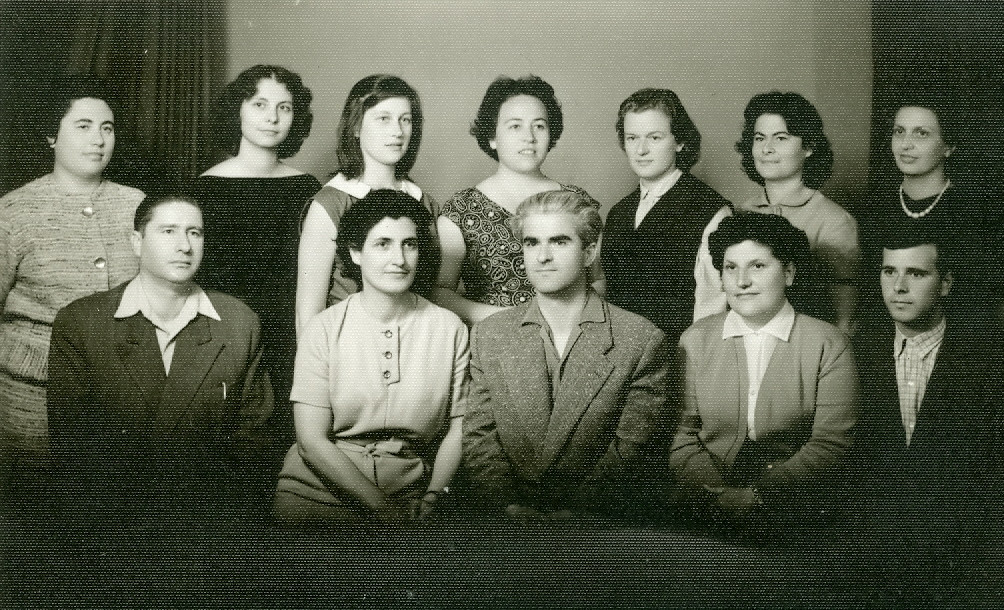
\includegraphics[width=4.4in]{./erste/1.jpg},\centerline{Първите учители}] \end{window}
През 1985г. гимназията е удостоена с орден „Кирил и Методий“.
От 1994 г. гимназията е първото училище в цяла Източна Европа със сертификат за 
езикова диплома (КМК ІІ), а от 1995г. училището е център за провеждане на изпити 
за България. Сертификатът за владеене на езика дава възможност на завършилите да 
постъпват в университети в Германия, Австрия и Швейцария без приемни изпити. 
Носители на този документ са много младежи и девойки, голяма част от които в 
настоящия момент са студенти в европейски университети.\\[0.1cm]
\\[7.5cm]От 1996г. училището разполага с модерна компютърна зала, включена и в Интернет. 
Изграденият с помощта на спонсори от гр. Дюселдорф информационен център по 
немски език, разполага с много и разнообразна справочна и художествена 
литература, технически средства и връзка с Интернет. 
% \columnbreak
През последните години тече младежки училищен обмен с партньори от Дюселдорф, 
Трабен - Трарбах. От 1998г. гимназия “Гьоте” е включена в европейския проект 
“Коменски” (Comenius-Project) и работи успешно със своите партньори от Румъния 
Полша, Швеция, Англия, Франция, Италия, Шотландия, Германия и Португалия. 
В гимназията се обучават около 800 ученика за 5 учебни години.  В 9-ти клас 
предметите биология и химия, а в 10-ти история, география,  се преподават изцяло 
на немски език.  От 2001г. директор на гимназията е г-жа Генета Илиева,  а от 
2011 г. директор е инж. Надежда Радева-Иванова.
На първа позиция е изучаването на немски език в гимназията, но в нея се изучава 
и разширено английски език, което позволява на учениците да участват в различни 
проекти. В гимназията има и новооткрита химична лаборатория, където могат да се 
правят експерименти и да се наблюдават биологични обекти под микроскоп. Актуални 
са и семинарите , които се предлагат на учениците .Учениците от гимназията 
печелят много конкурси, олимпиади, както и стипендиите на DAAD. 
\closearticle
\end{multicols}